\section{Overview of the LHCb software and data production}

The LHCb data production consists of the recording of the data by the LHCb detector, the processing of this data, and finally making the data available to physicists. In HEP analyses we also use the result of Monte Carlo simulations, which represent simulations of particle collisions. It is commonly used to help to characterize the signal (particle decay) of interest. These samples are kept in the same data format as the experimental (real) data and handled with the same software. In this paper, the term \emph{data} will be used to refer to both simulated data and the real experimental data.

The LHCb software is based on the Gaudi framework~\cite{barrand2001gaudi}. Gaudi is an object-oriented framework designed to provide a common infrastructure and environment for the different software applications of the LHCb experiment~\cite{corti2006software}. It is a modular software, which supports event data processing in real time inside the experiment, the data production in the offline system and the physics analyses performed by the users.

In each stage of the data production, we use a specialised software application. There are a number of versions of each application, in some cases over 100 different versions to date. Different versions can produce different physics output, thus making our data and physics results biased. Therefore it is crucial to know how the application manipulates the data in use. 


Initial stages of the Monte Carlo production~\cite{corti2015monte}:
\begin{itemize}
    \item \textbf{Simulation - Event generation.} The application {\it Gauss} mimics what happens inside the spectrometer of the LHCb experiment, simulating the initial data set of particle collisions~\cite{corti2006software}.
    \item \textbf{Digitization - Detector response.} The application {\it Boole} performs the simulation of the detector responses to produce the output in the same form as the experiment's electronics. 
    \item \textbf{L0 trigger emulation and  High level trigger (HLT).} Only a small fraction of the events produced in the LHCb detector are interesting to analyse. The trigger is a mechanism to select these events and save them, discarding the rest of the data (around 99\% of what was produced). The application that runs the triggers is {\it Moore}. Moore filters the simulated data in the same way as real data. 
\end{itemize}

The final stages in data production are the same for Monte Carlo samples as for the real data obtained by the data acquisition (DAQ) system (shown in Figures  \ref{fig:real} and \ref{fig:sim}). The settings in the applications are equivalent for both real data and simulation, to keep one consistent with the other:

\begin{itemize}
    \item \textbf{Turbo.} Turbo is a new streaming strategy where events are reconstructed in the trigger, thus bypassing the offline reconstruction and discarding the raw events~\cite{benson2015lhcb}. The application used in turbo stream, {\it Tesla}, writes out a compact summary of physics objects containing all the information necessary for analyses. 
    \item \textbf{Reconstruction.} In this stage, the detector hits are transformed into physics objects and written to disk. The {\it Brunel} application integrates the complete pattern recognition and produces files containing all reconstructed items such as calorimeter and trackers clusters, charged tracks and information on particle identification.
    \item \textbf{Streaming.} Streaming is the final stage of the production, which covers selection of the events. This is done with the {\it DaVinci} application~\cite{corti2006software}. \iffalse DaVinci is also used by the users doing analyses Hence, the output of the application can be purely statistical or event data. \fi
\end{itemize}


\iffalse 
\subsection{LHCb data production}

The experimental data is being recoded inside the LHCb detector. The expected detector output is obtained by computer simulation. We need the simulated data for the identification of particles and prediction of the detector behaviour. This data are often called Monte Carlo data. Both the experimental and simulated data go through the same production pipeline after they were created ~\cite{corti2006software}.

The data production pipeline is designed to maximise the data-taking efficiency and data quality. The pipeline consists of the following stages (figure 1), and at the each stage the input data is the product of the previous stage:

\begin{itemize}
    \item \textbf{Filtering data through the triggers.} This stage occurs while the data is being recorded inside the LHCb. Only a small fraction of the collisions inside the LHCb contain $B$ hadrons, and even a smaller fraction have interesting decays to study. If the triggers detect these decays, they will pass the data through, otherwise they will delete it. After selection in the fast hardware trigger, the data goes into the software triggers.
    \item \textbf{Reconstruction.} In this stage the detector hits are being transformed into objects such as particle tracks and clusters. The track fit determines the best estimate of the track parameters along the particle trajectory. We can obtain the momentum of the particle, position, direction etc. These objects are stored into an output file on disk.
    \item \textbf{Stripping.} The data is further filtered through a set of selections and more sophisticated track fits. This process reduces its size and makes it suitable and accessible to the users.
    \item \textbf{Users' analyses.} The users make their own cuts to the data and analyse it using their code.
\end{itemize}

\fi 
Figure \ref{fig:real} shows the real data production pipeline. After data acquisition in the {\it Online} system, the data is stored in RAW data format. It is further processed in \emph{Reconstruction} and \emph{Streaming} or \emph{Turbo} stages, before it is stored on a disk and made available to the physicists. 
Figure \ref{fig:sim} shows Monte Carlo simulation pipeline. The dice in the beginning of the pipeline represent a random generator, that is a central part of the simulation generation. The names of stages are followed by the names of applications used in each stage. 

\begin{figure}[h]
    \centering
    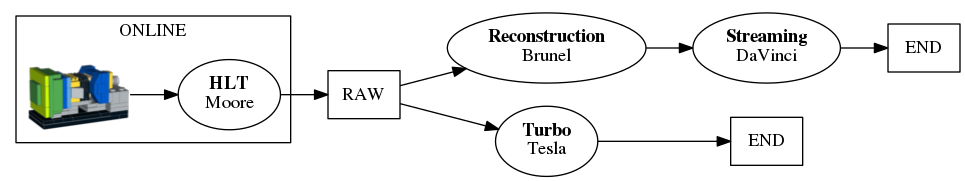
\includegraphics[width=\textwidth]{img/real}
    \caption{The real data production pipeline}
    \label{fig:real}
\end{figure}

\begin{figure}[h]
    \centering
    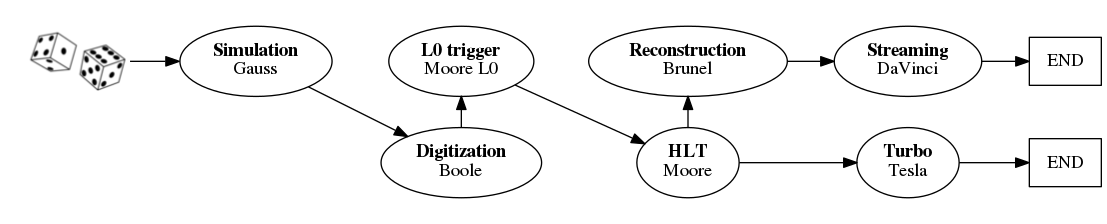
\includegraphics[width=\textwidth]{img/sim2}
    \caption{The simulation production pipeline}
    \label{fig:sim}
\end{figure}

\iffalse
\subsection{LHCb software stack}

The LHCb software stack is based on Gaudi framework~\cite{barrand2001gaudi}. It is modular software, which supports event data processing applications that run in real time high level triggers, the data and Monte Carlo production in the offline system and the physics analysis preformed by the users.

There are specialised software applications that are used in each of the stages. In some stages, such as creating simulated data, we use two different applications in the process. Different versions of an application can produce very different physics output, therefore it's crucial to know how the application manipulates the data in use. There are numerous versions of each of the applications, some of them reaching over 100 different versions.
\fi
